\documentclass[a4paper,man,natbib,floatsintext,donotrepeattitle]{apa6}

\usepackage[english]{babel}
\usepackage[utf8x]{inputenc}
\usepackage{amsmath}
\usepackage{graphicx}
\usepackage[colorinlistoftodos]{todonotes}
\usepackage{xcolor}
\usepackage[draft,inline,nomargin,index]{fixme}
\usepackage{hyperref}
\usepackage{verbatim}
\usepackage{nameref}
\usepackage{booktabs}
\usepackage{lineno}
\usepackage{amsfonts}
\usepackage{booktabs}
\usepackage{siunitx}
\linenumbers

\fxsetup{theme=color,mode=multiuser}
\FXRegisterAuthor{ab}{sab}{\color{blue}Amelie} % abnote{} with text inside to edit
\FXRegisterAuthor{bb}{sbb}{\color{purple}Brice} % bbnote{} with text inside to edit
\FXRegisterAuthor{ln}{sln}{\color{violet}Lad} % lnnote{} with text inside to edit

%\title{Blinding as a Necessary Precaution Against Experimenter Biases During Sequential Bayes Factor: A commentary on \cite{schonbrodt_sequential_2017}}

%\title{On the importance of blinding during sequential testing procedures: A commentary on \cite{schonbrodt_sequential_2017}}

%\title{"Efficient" yes, but only if you blind yourself: A commentary on \cite{schonbrodt_sequential_2017}}

%\title{"Efficient", but blind yourself as a precaution: A commentary on \cite{schonbrodt_sequential_2017}}

%Lad: je n'aime pas ce titre (ci-dessus)...l'anglais est maladroit...
%Brice: Oui

%\title{Blinding as a Precaution Against Experimenter Biases During Sequential Testing: A commentary on \cite{schonbrodt_sequential_2017}}

\title{Triple blinding for sequential testing: A commentary on \cite{schonbrodt_sequential_2017}}

\shorttitle{Blind Bayes Factor}
\threeauthors{Amélie G. Bret}{Brice Beffara}{Ladislas Nalborczyk}
\threeaffiliations{Univ. Grenoble Alpes, CNRS, LPNC, 38000, Grenoble, France \\Psychological Science Research Institute, Catholic University of Louvain, Belgium \\ The Walden III Slowpen Science Laboratory, France}{The Walden III Slowpen Science Laboratory, France}{Univ. Grenoble Alpes, CNRS, LPNC, 38000, Grenoble, France \\ Department of Experimental Clinical and Health Psychology, Ghent University \\ The Walden III Slowpen Science Laboratory, France}

\abstract{In this commentary we discuss potential issues associated with the Sequential Bayes Factor procedure as introduced by \cite{schonbrodt_sequential_2017}. We argue that particular precautions should be undertaken to ensure objectivity during sequential testing procedures (both Bayesian and frequentist). More precisely, we highlight the need for triple-blinding during such procedures, and provide recommendations on how to implement this without additional costs.}

\keywords{sequential testing, triple-blind, research methods}

% re-enabling section numbering (disabled by the apa6.csl)
% \setcounter{secnumdepth}{3}

\begin{document}

% defining a new command for counting words
\newcommand{\quickwordcount}{%
  \immediate\write18{texcount -1 -sum -merge \jobname.tex > \jobname-words.sum }%
  \input{\jobname-words.sum}words%
}

\maketitle

Wordcount: This document contains \textbf{\quickwordcount}.

\newpage

\tableofcontents % provisoire, juste pour se repérer entre nous
\newpage

% Notes
% répartition des tâches: Lad intro, Brice experimenter biases, Amélie blinding, et tout le monde section 3 et conclusion

%%%%%%%%%%%%%%%%%%%%%%%%%%%%%%%%%%%%%%%%
% début du comment
%%%%%%%%%%%%%%%%%%%%%%%%%%%%%

\newpage

\section{Introduction}

\cite{edwards_ward_bayesian_1963} state, "the rules governing when data collection stops are irrelevant to data interpretation. It is entirely appropriate to collect data until a point has been proven or disproven, or until the data collector runs out of time, money, or patience". However, as noted by \cite{schonbrodt_sequential_2017}, "this practice of unplanned multiple testing is not allowed in the classical NHST paradigm, because it increases Type I error rates". They add: "\textit{Of course, one can calculate statistics during data collection, but the results of these tests must not have any influence on optionally stopping data collection}."

We argue that such interim analysis (including visual inspections of the data) might have an influence on future data collection and optional stopping through overlooked experimenter biases, thus biasing the expected results of sequential testing procedures (both Bayesian and frequentist). While the procedure described in \cite{schonbrodt_sequential_2017} seems an attractive perspective and while we generally agree with most of their recommendations, we want to raise some concerns about precautions that need to be undertaken in order to preserve the long-terms rates of wrong inferences they provide. One major concern is that the person who runs the experiment and the person who analyses the data are usually the same person. As noted by \cite{wicherts_degrees_2016}, in the psychological field, "the analyses are typically conducted by a person who is not only aware of the hypotheses, but also benefits directly from corroborating them". Thus, failures of blinding procedures are listed among the 34 researchers degrees of freedom identified by \cite{wicherts_degrees_2016}. In the current commentary we will highlight the particular dramatic consequences of blinding failures in the context of sequential testing.

%Because we acknowledge and appreciate the importance of the seminal work of \cite{schonbrodt_sequential_2017}, in the second part of this commentary we highlight quick methodological precautions that will ensure the efficiency of the SBF procedure. 

%\todo{C'est surement parceque je parle pas bien anglais mais je trouve la formulation de cette phrase chelou, et lourde. }
%\lnnote{je suis complètement d'accord, et c'était redondant en plus}

%\subsection{The SBF design}

%In their paper, \cite{schonbrodt_sequential_2017} present an alternative to the much used NHST with a priori power analysis (NHST-PA). They introduce the \textit{Sequential Bayes Factor} (SBF) procedure that allows to collect data iteratively, until a predefined threshold is reached, while not suffering from the pitfalls associated with similar procedures used in the NHST framework. Testing mean differences between two independent groups, they show that the SBF design typically needs 50\% to 70\% smaller samples to reach a conclusion about the presence of an effect, as compared with optimal NHST-PA (where \textit{optimal} stands for an idealized situation in which the a priori targeted effect would be exactly equal to the \textit{true} effect size), while having similar long-term error rates.

%With this in mind, it is striking to see that though double blinding procedures have became a gold standard in many psychological fields, much less attention has been dedicated to triple blinding (i.e., procedures ensuring that the person who analyses the data is blinded to hypotheses).

\section{Intra and interpersonal biases in SBF procedure}

When a data analyst has expectations about what should be observed, data analysis is likely to be biased by these expectations trough confirmation (favoring an hypothesis) or disconfirmation (stronger skepticism toward data against the hypothesis than toward data corroborating the hypothesis) biases \citep{lilienfeld_blind_2017}. When an experimenter has expectations about what should be observed, data collection is likely to be biased by these expectations \citep{orne_social_1962,rosenthal_social_1963,rosenthal_experimenter_1964,tuyttens_opinion_2016,zoble_interaction_1969}.
In this comment, we discuss sequential testing assuming that both the participant and the experimenter are blind to the experimental condition (double blind design). In less rigorous conditions (simple blind or even no blinding at all), more problems can arise from sequential testing. \par

What is the specific status of sequential testing concerning analyst and observer expectancy effects ? Expectancy effects arise when one has prior believes and/or motivations about the issue of an experiment and unconsciously (we assume scientific honesty) influence the results on the basis of these prior believes and motivations. The confidence toward an hypothesis can be influenced by previous results from the literature, naive representations about the studied phenomenon, and all other sources of information. All these sources may deal with the studied phenomenon but never with the ongoing study specifically. As a consequence, the confidence about an hypothesis is always subject to uncertainty. When performing sequential testing, one has a direct access to accumulation of evidence concerning the ongoing study. As a consequence, the prior information is far more certain than previous studies or naive representations. Hence, the risk to fall into an "evidence confirmation" loop is not to be neglected. This risk applies both to confirmation and disconfirmation biases (data analysis), and observer expectancy effects (data collection). During data analysis, the intrapersonal bias of data evaluation can inflate with accumulated evidence. During data collection, the interpersonal bias of experimenter-participant interaction can inflate with accumulated evidence. However, the interpersonal bias is probably more important (more channels of influence), and we will therefore focus on it. \par

%\begin{figure}[H]
%  \caption{Overview of the SBF procedure and illustration of potential biases when the experimenter and the data analyst are the same person.}
%  \centering
%  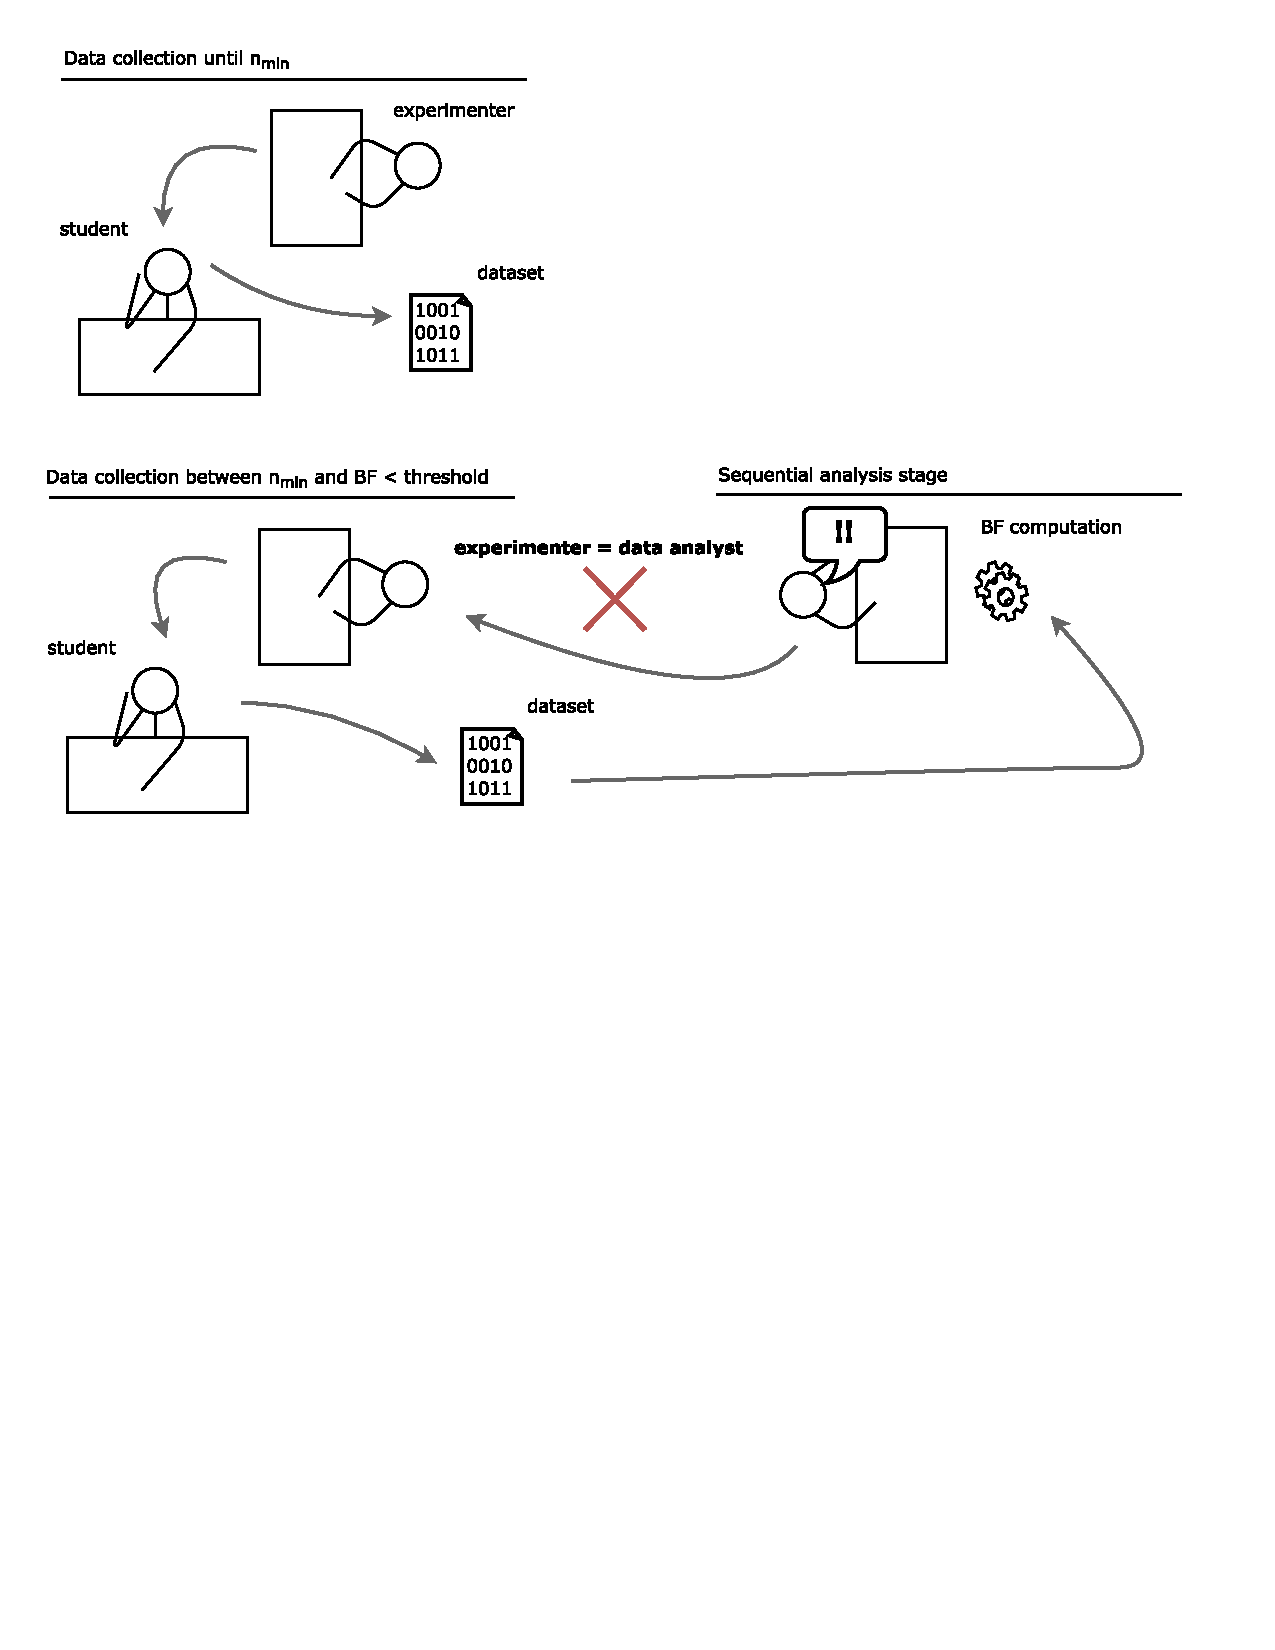
\includegraphics[width=0.8\textwidth]{figures/bias_diag.pdf}
%  \label{fig:diag1}
%\end{figure}

Obviously, It is very hard to obtain robust results concerning the effect size of analyst and observer expectancy effects. This "meta-science" problem is complicated because the biases can apply at all the levels as one experiment is included in another. It is also difficult to collect large observation sets by experimental conditions as we can note in \cite{zoble_interaction_1969}. Thus, we can only draw attention to these effects as a risk to consider rather than a robust and clear danger to avoid. \par

Because we assume a double blind design, how could knowledge about the data influence the issue of the experiment ? It is possible that the experimenter's verbal and non-verbal motor cues impact the participant's behavior \citep{zoble_interaction_1969}. Here the experimenter cannot influence the participant's responses on the basis of the experimental condition knowledge. However, we cannot exclude that the (de)motivation and the disappointment/satisfaction of seeing the preferred hypothesis contradicted/confirmed by the sequential testing procedure can influence the participant. We cannot exclude that the confidence in an hypothesis can interact with experimental conditions and impacts the issue of the experiment in one way or another.\par

Let's take a quick fictitious example. We want to study the effect of working memory (WM) training on math performance. We compare a WM training effect with a control group (e.g., short memory training) on a math test. Either in a between or a within participant design, let's imagine that there is a true effect of WM training on math performance (H1 is true). With accumulation of evidence in this direction, if the experimenter is not blind to sequential testing procedure (and let's say pro H1), it is likely that he or she will show higher enthusiasm when interacting with (e.g. delivering instruction to) the participant. The participant is in turn likely to want to perform the experiment at best \citep{zoble_interaction_1969}. The WM training is expected to increase performance at the math test. It is not impossible to observe an interaction between the motivation of the experimenter and the treatment effect, with increased motivation perceived during instructions explanations amplifying the positive effect of treatment. Importantly, there is no apparent reason that this kind of bias could not emerge in all combinations of motivation (see Table \ref{tab:pred}). \par

%\vline

%\begin{table}
%  \centering
%	\begin{tabular}{SSSS} \toprule
%     & \textbf{True} & & \\ 
%    \textit{Expected} & {effect} & \textit{H0} & \textit{H1} \\ \midrule
%     & \textbf{H0} & {+H0} & {-H0} \\
%     & \textbf{H1} & {-H1} & {+H1} \\ \bottomrule 
%	\end{tabular}
%    \caption{Possible interactions between true and expected effect on its %observation. + = accelerate and - = decelerate convergence.} %\label{tab:hexp}
%\end{table}
%\par

\vspace{5mm}

\begin{table}[H]
\centering
\caption{Possible interactions between true effect size and a priori beliefs on SBF. Congruent observations are expected to increase the speed of threshold reaching (H0+ and H1+), while incongruent observations are expected to slow down the process (H0- and H1-).}
\label{tab:pred}
\resizebox{\textwidth}{!}{%
\begin{tabular}{@{}ccc@{}}
\toprule
 & \begin{tabular}[c]{@{}c@{}}There is no difference in the population\\ (H0, d = 0)\end{tabular} & \begin{tabular}[c]{@{}c@{}}There is a difference in the population\\ (H1, e.g., d = 0.6)\end{tabular} \\ \midrule
Researcher 1, believes in H0 & H0+ (congruent) & H0- (incongruent) \\
Researcher 2, believes in H1 & H1- (incongruent) & H1+ (congruent) \\ \bottomrule
\end{tabular}%
}
\end{table}

Again, evidence is insufficient to conclude that analyst and observer expectancy effects are absolutely necessary to take into account. If the cost of reducing the bias was high, we could be skeptical about considering it knowing its uncertain benefits. However, as we will propose in the next section, very easy to implement and costless methods can be applied to overcome the expectancy problems. Hence, even with low certainty about the risks, it is worthwhile to limit it all the same. \par

% Sequential-Experimenter-Analyst-Bias (SEAB)...direct consequence of the SEAB is that it introduces a time dependency between participants...this kind of auto-correlated data would invalidate the use of the models compared by...in their original paper...

% \section{What does look like the SEAB ?}

These biases can wear a multitude of forms as it is a function of the researcher \textit{a-priori} expectancies and of the \textit{true} effect size. Moreover, we focus here on the simplest case in which the expectancies of the researcher remain constant throughout the sequential testing procedure. Although probably non realistic, this setting serves illustrative purposes in the next section. Figure \ref{fig:pred} illustrates our predictions for the four situations presented in Table \ref{tab:pred}.

\begin{figure}[H]
  \caption{Predicted consequences of the biases on the result of a SBF procedure with a fixed boundary of BF10 = 6 (or BF01 = 1/6), for a given Cohen's d of 0.5 (hereafter, "H1") or of 0 (hereafter "H0"), and according to the \emph{a priori} researcher beliefs.}
  \centering
  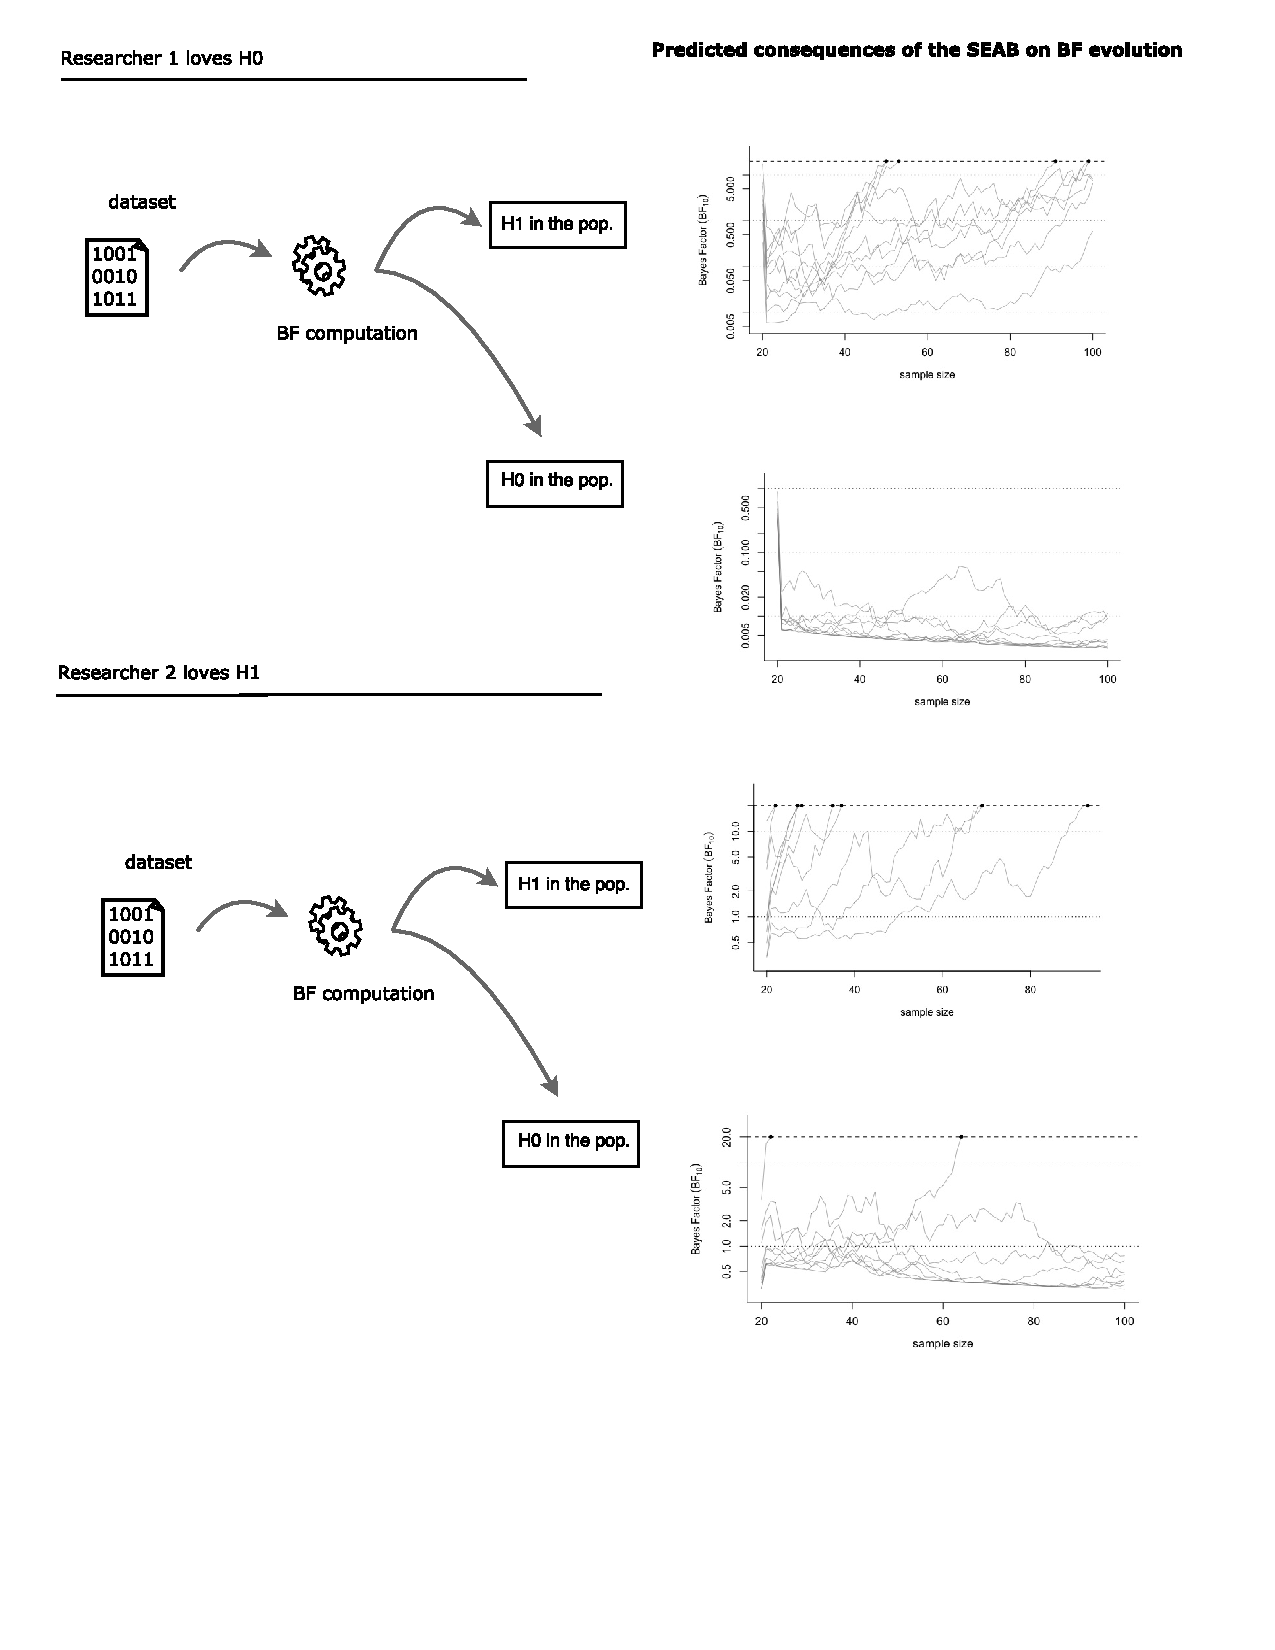
\includegraphics[width=0.8\textwidth]{figures/BFF_predictions.pdf}
  \label{fig:pred}
\end{figure}

% ajouter un paragraphe idée de amélie copiée par brice

According to these ideas, we suggest 1) two solutions that can be used as a precocious while we don't no the effect size of SEAB, 2) an experimental protocol in order to test the real impact of the experimenter with SBF. 

\section{Solutions ? Blind yourself.}

\subsection{Solution 1: one analyst, one experimenter}
The more we are able to blind ourself in experiment the best it could be (REF). Double blind is now the base line in psychology studies (REF), however, it does not allow to answer the problem of experimenter effect in the SBF procedure. So we suggest doing triple blind. But we know that it is a luxury possibility and it is not easy to apply, mostly due to materials and time constrains. \lnnote{est-ce que la solution 2 n'est pas aussi du triple blinding ?} \bbnote{A mon avis si ;-)} \abnote{Je ne pense pas, dans la solution 2 on traitera les données en conaissant les conditions}

\subsection{Solution 2: one analyst-experimenter, "software-blinded"}
If solution one is not possible we suggest a "software-blinded" solution. That is to say that the SBF function will only give the information of the quantity of evidence we have been collected but not the direction of this evidence. \lnnote{non, pas d'information sur la quantité d'evidence, juste "continues" ou arretes" le recrutement, cf. paragraphe suivant} \bbnote {tout à fait}
The huge point of this solution is the cost. We don't need to do a lot of effort to importantly improve the SBF advantages. 

\subsection{Full automation of data analysis}
When sequentially computing a BF, we have to make choices about how we deal with data. Indeed, based on previous studies, we have expectations about the range of plausible values, need for data re-coding or transforming, the distribution of residuals, and so on. All these decisions have to be made before BF computing in order to obtain reliable evidence toward an hypothesis. In a triple blind perspective, we propose that all the data analysis steps needed before BF computing should also be automated and performed at each step of the sequential testing. This should prevent the data analyst from classical traps during data manipulation. Theses traps could be more dramatic in SBF versus traditional procedures due to the incremental expectancy effect. Besides, it fits with the open science philosophy and especially with preregistrations practices. Indeed, we propose that the code performing the SBF should also contain all the other data analysis steps needed. These steps would be programmed and coded on the basis of choices preregistered before the beginning of data collection. Triple blind designs with automated data analysis would therefore increase the strength of SBF for diminishing error rates and explicitly fulfill the requirements of clean open science. \par

In order to process with this, we added a very short append to the \texttt{seqBF} function, written by Félix Schönbrodt \& Richard Morey (available \href{https://raw.githubusercontent.com/richarddmorey/BayesFactorExtras/master/BayesFactorExtras/R/seqBF.R}{here}), so that the user can now simply set the \texttt{blind} argument to \texttt{TRUE} and thus be completely blind to the results of the sequential BF computations. The only output is a sentence that either indicates to "continue" or to "stop" the recruitment, considering an a-priori defined threshold (see \nameref{sec:supp} for code details).

%\subsection{Experimental demonstration}
%After Rosenthal's studies, the effect of experimenter influence in the experiment have not been studied a lot. Because of this lack of knowledge, and of the hypothetical importance in the SBF, we suggest a simple design to test the experimenter bias. Following the Figure 2. In one condition, we would say the experimenter that the effect is congruent with H0... One group without any SEAB correction, and the second one with a triple blind or a software-blind. 

\section{Conclusions}

With this comment we would like to point out the importance of SBF procedure when it is compiled with a blinding procedure. We agree that only few and non recent papers are highlighted experimenters bias, but we think that we can not take the risk with a so highly rigorous procedure to add any social bias. Doing both of those procedure (SBF and blinding) could, in our view, increase again the quality of the transparency and the rigor of research. 

% exemple de manip utilisant le SBF: \cite{martin_perceiving_2016}

\section{Supplementary materials}\label{sec:supp}

Reproducible code and supplementary materials can be found on OSF: \url{osf.io/mwtvk
}.

\section{Acknowledgements}

...

\bibliography{BBF_BFF}

Rosenthal, R. (1966). Experimenter effects in behavioral research. East Norwalk, CT: Appleton-Century-Crofts.

Harris, M. J., and Rosenthal, R. (1985). Mediation of interpersonal expectancy
effects: 31 meta-analyses. Psychological Bulletin, 97(3), 363-386.

\lnnote{à ajouter au .bib}

\end{document}
